\begin{problem}[18]
讨论悬臂梁在自重作用下的最大挠度与梁长的关系.
\end{problem}
% --------------------------------------------------------------------
\begin{solution}
\begin{minipage}[c]{0.7\linewidth}
该问题的控制参数有: 梁的长度$l$, 梁的抗弯刚度$EI$($E$为杨氏模量, $I$为截面矩), 单位长度梁重$q$, 于是最大挠度应该是上述参数的函数:
\[
w_{\max} = f(l; EI; q)
\]
\end{minipage}
\begin{minipage}[c]{0.3\linewidth}
\begin{center}
\usetikzlibrary{calc,intersections,through,backgrounds}
\usetikzlibrary{decorations.pathreplacing,decorations.pathmorphing,arrows}
\usetikzlibrary{shapes}
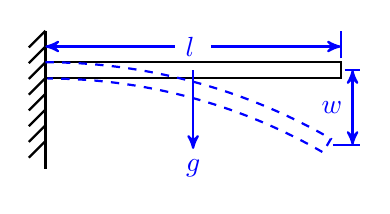
\begin{tikzpicture}[interface/.style={
        postaction={draw,decorate,decoration={border,angle=-45,
                    amplitude=0.3cm,segment length=2mm}}}]
\draw[interface,thick] (0,0.5)--(0,-1.25);
\draw [thick] (0,-0.1) rectangle (3.75,0.1);
\draw [thick,blue,dashed] (0,0.1) arc (90:60:7.25 and 7.25) --++(-0.1,-0.17321)  arc (60:90:7 and 7) ;
\draw [thick,blue,->,>=stealth'](1.875,0)--(1.875,-1) node[below]{$g$};

\draw[thick,blue,<->,>=stealth'] (3.65,-0.95)--(4,-0.95) (3.8,0)--(4,0) (3.9,0)--(3.9,-0.95) node[midway,left]{$w$};

\draw[blue,thick,<-,>=stealth'](3.75,0.15) -- (3.75,0.5) (0,0.3)--(1.65,0.3) node [right]{$l$};
\draw[blue,thick,->,>=stealth'](2.1,0.3)--(3.75,0.3);
\end{tikzpicture}
\end{center}
\end{minipage}\vspace{10pt}

上式中各物理量的量纲分别为: $[w_{\max}]=[l]=L$, $[EI]=FL^2$, $q=FL^{-1}$. 该问题中含两个独立量纲, 取$l$和$EI$作为基本量, 且组成单位系统, 于是上式可转化为
\[
\frac{w_{\max}}{l} = f\bigg(1,1,\frac{q}{EI/l^3}\bigg) 
\quad\Longrightarrow\quad
w = l f\bigg(\frac{ql^3}{EI}\bigg) 
\]
考虑到在弹性范围内有$w_{\max}\propto 1/E$, 与上式对比可得
\[
w_{\max} = C\frac{q}{EI} l^4
\]
其中$C$为常数, 可见悬臂梁在自重作用下的最大挠度$w_{\max}$与梁长的四次方$l^4$成正比.
\end{solution}
